\section{Experimental Results and Evaluation}\label{sec:results}

This section evaluates the effectiveness and generalization of \scl{} against the host trackers
using identical detections and published tracker configurations. Section~\ref{sec:tracker}
examines tracking performance across different trackers on MOT17, while Sect.~\ref{sec:detector}
evaluates detector--tracker compatibility on KITTI. Section~\ref{sec:shift} investigates robustness
to detection confidence-score shifts, and Sect.~\ref{sec:baselines} compares \scl{} with adaptive
thresholding methods. Section~\ref{sec:ablation} presents component ablation and parameter
sensitivity analyses. Finally, Sects.~\ref{sec:external} and~\ref{sec:visdrone} assess
generalization to previously unseen trackers and the held-out UAVDT dataset, respectively. In all
comparisons, the baseline is the host tracker operating without \scl{}, and Fig.~\ref{fig:forest}
summarizes the HOTA differences across the evaluated configurations.

\emph{How to read the result tables.} Each row gives one metric of the tracker alone (Host) and
with \scl{} (Host+\scl{}), and Change with its 95\% interval (Sect.~\ref{sec:metrics}); a bold change
is reliable, and ``identical'' means an unchanged output. For example, in Table~\ref{tab:mot17},
OC-SORT at floor 0.01 has a MOTA of 74.67 alone and 75.94 with \scl{}: the change is $+1.27$ points,
and its interval $[+0.17,+3.01]$ lies above zero, so the gain is reliable.
Values are rounded separately, so Host+\scl{} minus Host can differ from Change in the last digit.

\begin{figure}[!t]
\centering
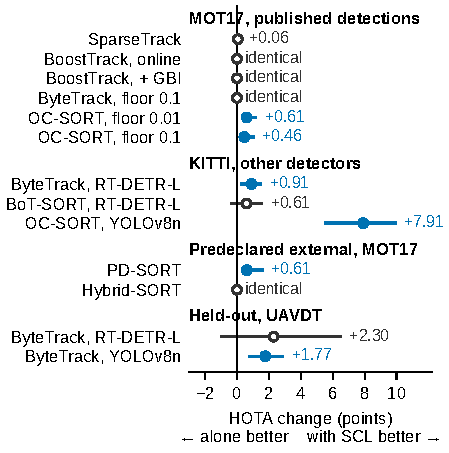
\includegraphics{Fig3.pdf}
\caption{HOTA change with \scl{} (tracker with \scl{} minus tracker alone, in points) for the
tested trackers and detectors. Dot and number: the change; line: its 95\% bootstrap interval; right
of zero, \scl{} is better. Filled dot: a reliable gain; open dot: no reliable change or identical
output}
\label{fig:forest}
\end{figure}

\subsection{Performance Across Trackers on MOT17}\label{sec:tracker}
Table~\ref{tab:mot17} shows the development trackers on MOT17 val-half. The two-stage trackers with
well-matched detections kept the accuracy of their hosts: BoostTrack, online and with GBI, and
ByteTrack at floor 0.1 gave exactly the same output, and SparseTrack rose by 0.06 HOTA points
through the self-limiting clean mode. The single-stage OC-SORT improved at both floors (HOTA from
66.43 to 67.04 and from 66.44 to 66.91, MOTA $+1.27$ and $+1.26$), with fewer identity switches and
higher HOTA on 7 of 7 sequences, through the continuation rescue.

\begin{table}[!tb]
\caption{MOT17 val-half, published YOLOX-X detections: each development tracker alone (Host) and with \scl{} (Host+\scl{}). Change: Host+\scl{} minus Host, with its 95\% bootstrap interval; bold: a reliable change. Paper: the value reported by the tracker's authors (--: not reported). Floor: the lowest emitted detector score.}
\label{tab:mot17}
\centering\footnotesize
\setlength{\tabcolsep}{2.5pt}
\begin{tabular}{@{}lrrrl@{}}
\toprule
Metric & Paper & Host & \begin{tabular}[b]{@{}r@{}}Host\\+\scl{}\end{tabular} & Change [95\% CI]\\
\midrule
\multicolumn{5}{@{}l}{\textit{SparseTrack} \cite{liu2025sparsetrack}}\\
\quad HOTA$\uparrow$ & 69.2 & 68.88 & 68.93 & $+0.06$ [$-0.01$, $+0.25$]\\
\quad MOTA$\uparrow$ & 76.8 & 77.85 & 77.93 & $+0.08$ [$-0.03$, $+0.30$]\\
\quad IDF1$\uparrow$ & 81.4 & 81.97 & 82.13 & $+0.16$ [$-0.02$, $+0.70$]\\
\multicolumn{5}{@{}l}{\textit{BoostTrack, online} \cite{stanojevic2024boosttrack}}\\
\quad HOTA$\uparrow$ & 68.37 & 68.49 & 68.49 & 0 (identical)\\
\quad MOTA$\uparrow$ & 75.56 & 75.50 & 75.50 & 0 (identical)\\
\quad IDF1$\uparrow$ & 81.35 & 81.41 & 81.41 & 0 (identical)\\
\quad IDS$\downarrow$ & 118 & 113 & 113 & 0 (identical)\\
\multicolumn{5}{@{}l}{\textit{BoostTrack, + GBI} \cite{stanojevic2024boosttrack}}\\
\quad HOTA$\uparrow$ & 71.33 & 71.73 & 71.73 & 0 (identical)\\
\quad MOTA$\uparrow$ & 80.55 & 81.03 & 81.03 & 0 (identical)\\
\quad IDF1$\uparrow$ & 83.84 & 84.16 & 84.16 & 0 (identical)\\
\quad IDS$\downarrow$ & 106 & 97 & 97 & 0 (identical)\\
\multicolumn{5}{@{}l}{\textit{ByteTrack, floor 0.1} \cite{zhang2022bytetrack}}\\
\quad HOTA$\uparrow$ & -- & 67.70 & 67.70 & 0 (identical)\\
\quad MOTA$\uparrow$ & 76.6 & 77.60 & 77.60 & 0 (identical)\\
\quad IDF1$\uparrow$ & 79.3 & 79.47 & 79.47 & 0 (identical)\\
\quad IDS$\downarrow$ & -- & 214 & 214 & 0 (identical)\\
\multicolumn{5}{@{}l}{\textit{OC-SORT, floor 0.01} \cite{cao2023ocsort}}\\
\quad HOTA$\uparrow$ & 66.5 & 66.43 & 67.04 & {\boldmath $+0.61$ [$+0.36$, $+1.24$]}\\
\quad MOTA$\uparrow$ & 74.9 & 74.67 & 75.94 & {\boldmath $+1.27$ [$+0.17$, $+3.01$]}\\
\quad IDF1$\uparrow$ & 77.7 & 78.05 & 78.71 & $+0.66$ [$-0.25$, $+1.60$]\\
\quad IDS$\downarrow$ & -- & 211 & 203 & {\boldmath $-8$ [$-15$, $-2$]}\\
\multicolumn{5}{@{}l}{\textit{OC-SORT, floor 0.1} \cite{cao2023ocsort}}\\
\quad HOTA$\uparrow$ & 66.5 & 66.44 & 66.91 & {\boldmath $+0.46$ [$+0.27$, $+1.09$]}\\
\quad MOTA$\uparrow$ & 74.9 & 74.67 & 75.93 & {\boldmath $+1.26$ [$+0.37$, $+3.34$]}\\
\quad IDF1$\uparrow$ & 77.7 & 78.05 & 78.33 & {\boldmath $+0.287$ [$+0.003$, $+0.838$]}\\
\quad IDS$\downarrow$ & -- & 213 & 199 & $-14$ [$-38$, $+6$]\\
\bottomrule
\end{tabular}
\end{table}


\subsection{Cross-Detector Evaluation on KITTI}\label{sec:detector}
Table~\ref{tab:kitti} shows what happens when the detector is replaced. With the noisy RT-DETR-L,
\scl{} raised ByteTrack by 5.98 MOTA, 3.87 IDF1, and 0.91 HOTA points and BoT-SORT by 7.86 MOTA,
3.10 IDF1, and 0.61 HOTA points, with 297 and 226 fewer identity switches. With YOLOv8n, OC-SORT
rose from 36.27 to 44.18 HOTA ($+7.91$ points, $[+5.47,+9.98]$), 9.40 MOTA points, and 9.60 IDF1
points, as its missed objects (FN) fell by 5,310. Fig.~\ref{fig:example} follows this cell over
three frames: each object keeps its ID, and at frame 102 OC-SORT alone tracked 6 of the 10 labelled
objects and with \scl{} 9.

\begin{figure*}[t]
\centering
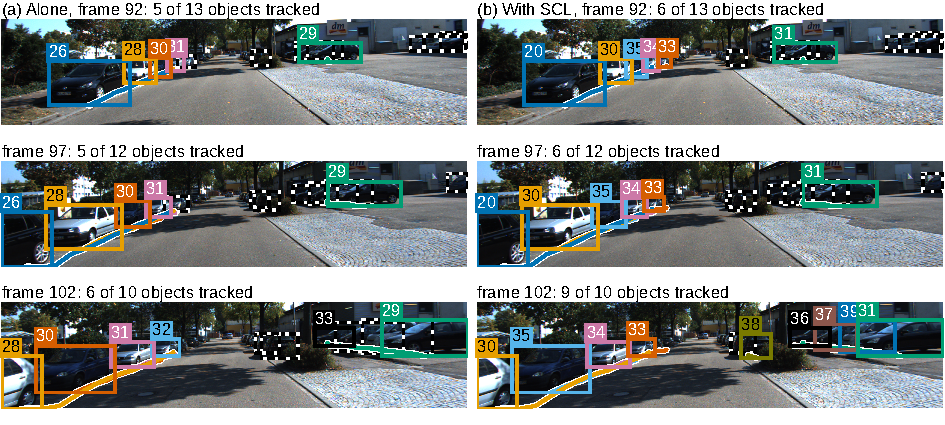
\includegraphics{Fig4.pdf}
\caption{KITTI sequence 0001 \cite{geiger2012kitti} tracked by OC-SORT with YOLOv8n at frames 92,
97, and 102 (rows): (a) the tracker alone; (b) with \scl{}. Each colour and number is one track; its
line shows the object's last 20 frames. Dashed boxes: labelled objects that no track follows. IDs
are numbered separately in each run. The sequence has the median HOTA gain of the 21 sequences, and frame 102 is
its first frame with the largest gain in tracked objects}
\label{fig:example}
\end{figure*}

\begin{table}[!tb]
\caption{KITTI tracking training with detectors the trackers were not tuned for (HOTA averaged over cars and pedestrians); columns as in Table~\ref{tab:mot17}. BoT-SORT leaves out sequence 0020 in both runs, because its code stops with a numerical error on it.}
\label{tab:kitti}
\centering\footnotesize
\setlength{\tabcolsep}{2.5pt}
\begin{tabular}{@{}lrrl@{}}
\toprule
Metric & Host & \begin{tabular}[b]{@{}r@{}}Host\\+\scl{}\end{tabular} & Change [95\% CI]\\
\midrule
\multicolumn{4}{@{}l}{\textit{ByteTrack} \cite{zhang2022bytetrack}\textit{, RT-DETR-L}}\\
\quad HOTA$\uparrow$ & 50.73 & 51.64 & {\boldmath $+0.91$ [$+0.22$, $+1.55$]}\\
\quad MOTA$\uparrow$ & 47.27 & 53.24 & {\boldmath $+5.98$ [$+1.16$, $+9.94$]}\\
\quad IDF1$\uparrow$ & 64.98 & 68.86 & {\boldmath $+3.87$ [$+1.67$, $+5.06$]}\\
\quad IDS$\downarrow$ & 686 & 389 & {\boldmath $-297$ [$-530$, $-122$]}\\
\multicolumn{4}{@{}l}{\textit{BoT-SORT} \cite{aharon2022botsort}\textit{, RT-DETR-L} (20 sequences)}\\
\quad HOTA$\uparrow$ & 53.91 & 54.52 & $+0.61$ [$-0.39$, $+1.61$]\\
\quad MOTA$\uparrow$ & 48.25 & 56.11 & {\boldmath $+7.86$ [$+2.21$, $+13.44$]}\\
\quad IDF1$\uparrow$ & 67.74 & 70.85 & {\boldmath $+3.10$ [$+1.00$, $+4.57$]}\\
\quad IDS$\downarrow$ & 476 & 250 & {\boldmath $-226$ [$-369$, $-120$]}\\
\multicolumn{4}{@{}l}{\textit{OC-SORT} \cite{cao2023ocsort}\textit{, YOLOv8n}}\\
\quad HOTA$\uparrow$ & 36.27 & 44.18 & {\boldmath $+7.91$ [$+5.47$, $+9.98$]}\\
\quad MOTA$\uparrow$ & 33.99 & 43.39 & {\boldmath $+9.40$ [$+1.10$, $+12.30$]}\\
\quad IDF1$\uparrow$ & 50.46 & 60.05 & {\boldmath $+9.60$ [$+5.61$, $+12.16$]}\\
\bottomrule
\end{tabular}
\end{table}


\subsection{Robustness to Detection Score Shifts}\label{sec:shift}
Table~\ref{tab:shift} shows the trackers under the four score transforms. Halving the scores
reduced ByteTrack (official setting) and OC-SORT to 0 HOTA; with the layer they reached 66.17 and
66.72. Cubing reduced them to 60.92 and 58.34, and the layer restored them to 65.81 and 66.60;
BoostTrack rose from 61.33 to 64.84. With $T=2$, the layer raised ByteTrack and OC-SORT by 1.11 and
1.24 points. Across the score changes, the layer raised HOTA significantly in 7 conditions.

\begin{table}[!tb]
\caption{MOT17 val-half with the detector scores changed before the tracker, which keeps its published thresholds: $s^3$ cubes every score, $0.5\,s$ halves it, and $T=2$ and $T=0.5$ divide its logit by 2 or 0.5. HOTA of the tracker alone (Host) and with \scl{} (Host+\scl{}); 0.00: no object tracked; Change with its 95\% bootstrap interval; bold: a reliable change. Lowest emitted score 0.01 (BoostTrack 0.1).}
\label{tab:shift}
\centering\footnotesize
\setlength{\tabcolsep}{3pt}
\begin{tabular}{@{}lrrl@{}}
\toprule
 & \multicolumn{3}{c}{HOTA (\%)}\\
\cmidrule(l){2-4}
Score change & Host & \begin{tabular}[b]{@{}r@{}}Host\\+\scl{}\end{tabular} & Change [95\% CI]\\
\midrule
\multicolumn{4}{@{}l}{\textit{ByteTrack, official setting} \cite{zhang2022bytetrack}}\\
\quad $s^3$ & 60.92 & 65.81 & {\boldmath $+4.89$ [$+2.60$, $+13.69$]}\\
\quad $0.5\,s$ & 0.00 & 66.17 & {\boldmath $+66.17$ [$+49.32$, $+75.40$]}\\
\quad $T=2$ & 65.84 & 66.95 & {\boldmath $+1.11$ [$+0.35$, $+3.87$]}\\
\multicolumn{4}{@{}l}{\textit{OC-SORT} \cite{cao2023ocsort}}\\
\quad $s^3$ & 58.34 & 66.60 & {\boldmath $+8.26$ [$+5.86$, $+16.81$]}\\
\quad $0.5\,s$ & 0.00 & 66.72 & {\boldmath $+66.72$ [$+50.32$, $+75.56$]}\\
\quad $T=2$ & 65.99 & 67.22 & {\boldmath $+1.24$ [$+0.52$, $+3.42$]}\\
\quad $T=0.5$ & 66.61 & 67.06 & $+0.45$ [$-0.01$, $+0.97$]\\
\multicolumn{4}{@{}l}{\textit{BoostTrack, online} \cite{stanojevic2024boosttrack}}\\
\quad $s^3$ & 61.33 & 64.84 & {\boldmath $+3.51$ [$+0.85$, $+13.28$]}\\
\quad $T=2$ & 67.59 & 67.59 & 0 (identical)\\
\bottomrule
\end{tabular}
\end{table}


\subsection{Comparison with Adaptive Thresholding Methods}\label{sec:baselines}
Two simple baselines set the tracker's matching and birth thresholds in every frame to the first or
second Otsu split of the logits of the last 10 frames, $t_1$ or $t_2$, and pass the scores
unchanged. On KITTI (Table~\ref{tab:baselines}), \scl{} reached the highest HOTA in all three
cells, 2.2 to 8.6 points above the baselines, with intervals against the $t_2$ baseline above zero
in every cell, so adaptive thresholds alone do not explain the gains.

\begin{table}[!tb]
\caption{KITTI tracking training: HOTA of the tracker alone (Host), of two adaptive baselines that set the tracker's thresholds in every frame to the first ($t_1$) or second ($t_2$) Otsu split of the logits of the last 10 frames, and of \scl{}. Halved: halved detector scores. \scl{} $-$ $t_2$: the gain over the stronger baseline, with its 95\% bootstrap interval below; bold: a reliable gain.}
\label{tab:baselines}
\centering\footnotesize
\setlength{\tabcolsep}{3pt}
\begin{tabular}{@{}lrrrrc@{}}
\toprule
Cell & Host & $t_1$ & $t_2$ & \scl{} & \scl{} $-$ $t_2$\\
\midrule
\twol{OC-SORT,}{YOLOv8n} & 36.27 & 39.97 & 41.09 & 44.18 & \cib{+3.09}{+2.00}{+4.03}\\
\addlinespace[3pt]
\begin{tabular}[c]{@{}l@{}}ByteTrack,\\RT-DETR-L,\\halved\end{tabular} & 49.50 & 49.58 & 49.50 & 51.79 & \cib{+2.29}{+0.28}{+4.96}\\
\addlinespace[3pt]
\begin{tabular}[c]{@{}l@{}}OC-SORT,\\YOLOv8n,\\halved\end{tabular} & 0.00 & 37.68 & 43.56 & 46.30 & \cib{+2.74}{+1.32}{+3.34}\\
\bottomrule
\end{tabular}
\end{table}


\emph{Logit-to-score conversion.} The splits are found on logits and converted to scores with the
logistic function; the thresholds recorded in every frame equalled the intended values, $\sigma(t_1)$
or $\sigma(t_2)$ in all eight baseline runs, and $\min(a,\sigma(t_2))$ (Eq.~\eqref{eq:clean}) or 0.5
in the four KITTI cells of \scl{}.

\emph{ACT.} ACT \cite{act2026adaptive}, the closest published method (Sect.~\ref{sec:survey}), was run with its published parameters on the same detections and hosts as
\scl{} (Table~\ref{tab:act}): its high threshold became the host's matching threshold (with OC-SORT,
its single threshold) and its low threshold the lower bound of the second step. With the host's own
thresholds, the ACT runner reproduced the host exactly in all 84 KITTI, 14 MOT17, and 40 UAVDT
sequence runs.

\begin{table*}[!tp]
\caption{ACT \cite{act2026adaptive}, with its published parameters, and \scl{} on the same detections and tracker. (a) HOTA with each method, and \scl{} $-$ ACT in HOTA and IDF1 with its 95\% bootstrap interval. (b) MOTA and identity switches on UAVDT. A positive HOTA, IDF1, or MOTA difference and a negative IDS difference favour \scl{}; bold: a reliable difference. KITTI: HOTA averaged over cars and pedestrians; MOT17: val-half, the setting ACT was designed for; UAVDT: test split.}
\label{tab:act}
\centering\footnotesize
\setlength{\tabcolsep}{3pt}
{\textit{(a) HOTA and IDF1}}\par\smallskip
\begin{tabular}{@{}lllrrll@{}}
\toprule
Data & Detector & Tracker & ACT & \scl{} & \scl{} $-$ ACT, HOTA [95\% CI] & \scl{} $-$ ACT, IDF1 [95\% CI]\\
\midrule
KITTI, halved & RT-DETR-L & ByteTrack & 49.77 & 51.79 & {\boldmath $+2.01$ [$+0.01$, $+4.76$]} & $+1.70$ [$-1.13$, $+6.80$]\\
KITTI, halved & YOLOv8n & OC-SORT & 36.24 & 46.30 & {\boldmath $+10.06$ [$+6.88$, $+12.01$]} & {\boldmath $+12.03$ [$+6.85$, $+14.69$]}\\
\addlinespace[2pt]
MOT17, floor 0.01 & YOLOX-X & ByteTrack (official) & 67.46 & 67.68 & $+0.22$ [$-0.43$, $+0.88$] & $+0.57$ [$-0.68$, $+2.12$]\\
MOT17, floor 0.1 & YOLOX-X & ByteTrack (official) & 67.46 & 67.70 & $+0.23$ [$-0.40$, $+0.90$] & $+0.60$ [$-0.55$, $+2.10$]\\
\addlinespace[2pt]
UAVDT test & YOLOv8n & ByteTrack & 29.01 & 30.83 & {\boldmath $+1.82$ [$+0.65$, $+3.00$]} & {\boldmath $+4.00$ [$+1.85$, $+6.22$]}\\
UAVDT test & RT-DETR-L & ByteTrack & 40.14 & 42.37 & $+2.23$ [$-0.97$, $+6.32$] & $+5.35$ [$-0.03$, $+12.47$]\\
\bottomrule
\end{tabular}

\medskip
{\textit{(b) MOTA and identity switches on UAVDT (test split, ByteTrack)}}\par\smallskip
\begin{tabular}{@{}lrrlrrl@{}}
\toprule
 & \multicolumn{3}{c}{MOTA$\uparrow$} & \multicolumn{3}{c}{IDS$\downarrow$}\\
\cmidrule(lr){2-4}\cmidrule(l){5-7}
Detector & ACT & \scl{} & \scl{} $-$ ACT [95\% CI] & ACT & \scl{} & \scl{} $-$ ACT [95\% CI]\\
\midrule
YOLOv8n & 16.59 & 17.29 & $+0.71$ [$-1.42$, $+2.52$] & 578 & 393 & $-185$ [$-480$, $+13$]\\
RT-DETR-L & 5.34 & 27.99 & {\boldmath $+22.65$ [$+9.03$, $+47.21$]} & 873 & 455 & {\boldmath $-418$ [$-718$, $-123$]}\\
\bottomrule
\end{tabular}
\end{table*}


\scl{} reached
higher HOTA than ACT in every row of Table~\ref{tab:act}a, significantly under halved scores
($+2.01$ and $+10.06$ points) and with YOLOv8n on UAVDT ($+1.82$), and also in the MOT17 setting for
which ACT was designed. On UAVDT (Table~\ref{tab:act}b), \scl{} also reached a higher MOTA and had
fewer identity switches than ACT with both detectors; with RT-DETR-L its MOTA was 27.99 against 5.34
($+22.65$, $[+9.03,+47.21]$), with 418 fewer identity switches, because the fixed score levels of
ACT removed few of the host's false positives.

\subsection{Component Ablation and Parameter Sensitivity}\label{sec:ablation}
Table~\ref{tab:compabl} removes one part of the frozen \scl{}, or changes one of its values, at a
time on the three KITTI cells of Table~\ref{tab:baselines}. Each part matters where its step acts.
Without the weak detection recovery, the single-stage OC-SORT lost up to 3.35 HOTA points, as it has
no low-score step of its own; without the noisy mode (always clean), the halved-score cells lost up
to 2.44 points, without the remap up to 1.67, and without the motion tolerance up to 0.14. The clean
mode, in turn, keeps well-matched trackers at their own accuracy (Table~\ref{tab:prior}).

\begin{table}[!tb]
\caption{What each part and each fixed value of \scl{} contributes on the three KITTI cells of Table~\ref{tab:baselines} (HOTA): (a) OC-SORT, YOLOv8n; (b) ByteTrack, RT-DETR-L, halved scores; (c) OC-SORT, YOLOv8n, halved scores. Middle: one part removed at a time, with the largest HOTA loss and its cell. Lower: one fixed value changed at a time (frozen value in brackets), with the largest HOTA change over the tested values and cells.}
\label{tab:compabl}
\centering\footnotesize
\setlength{\tabcolsep}{3pt}
\begin{tabular}{@{}lrc@{}}
\toprule
\multicolumn{3}{@{}l}{Frozen \scl{}, HOTA: (a) 44.18, (b) 51.79, (c) 46.30}\\
\midrule
Part removed & Largest loss & Cell\\
\midrule
Weak detection recovery & 3.35 & (a)\\
Noisy mode (always clean) & 2.44 & (c)\\
Remap (raw scores) & 1.67 & (b)\\
Motion tolerance & 0.14 & (c)\\
\midrule
Value changed (frozen) & Largest change & Tested\\
\midrule
Window $W$ (10 frames) & 0.56 & 5, 20\\
Mode median frames (all) & 0.36 & last 100, 300\\
Duplicate/recovery IoU (0.5) & 0.62 & 0.4, 0.6\\
Motion history (100 frames) & 0.09 & 50, 200\\
\bottomrule
\end{tabular}
\end{table}


The sensitivity analysis, planned before the runs, changed the window $W$, the frames whose median
decides the mode, the IoU of the duplicate and recovery rules, and the motion history. For every
value and cell, HOTA stayed within 0.62 points of the frozen \scl{}, and within 0.24 points on a
fourth cell, ByteTrack with the original RT-DETR-L scores. None of the values thus needs tuning for
these detectors and trackers.

\subsection{Generalization to Unseen Trackers}\label{sec:external}
Table~\ref{tab:external}a gives the two predeclared external systems. PD-SORT \cite{wang2025pdsort}
was reproduced exactly; with \scl{}, its HOTA rose from 68.01 to 68.62 ($+0.61$ points,
$[+0.27,+1.65]$), its MOTA by 1.13 ($[+0.27,+3.03]$), and its IDF1 by 0.82 ($[+0.43,+1.94]$), with
higher HOTA on 7 of 7 sequences. Like OC-SORT, it is a single-stage tracker, but it was not seen
during design. Hybrid-SORT \cite{yang2024hybridsort}, a two-stage tracker, gave identical output, as
predicted before the run.

\begin{table}[!tb]
\caption{Generalization, each run once with the frozen \scl{}; columns as in Table~\ref{tab:mot17}. (a) The two external trackers, chosen before the run and not used during design (MOT17 val-half, the authors' detections); Paper: the authors' number (for PD-SORT, their released output); EXACT: Host within 0.2 HOTA of it; CLOSE: within 1.0. (b) The held-out UAVDT test split (20 drone videos, not used during design), ByteTrack with its published setting.}
\label{tab:external}
\centering\footnotesize
\setlength{\tabcolsep}{2.5pt}
\begin{tabular}{@{}lrrrl@{}}
\toprule
Metric & Paper & Host & \begin{tabular}[b]{@{}r@{}}Host\\+\scl{}\end{tabular} & Change [95\% CI]\\
\midrule
\multicolumn{5}{@{}l}{(a) \textit{PD-SORT} \cite{wang2025pdsort}\textit{, EXACT}}\\
\quad HOTA$\uparrow$ & 68.01 & 68.01 & 68.62 & {\boldmath $+0.61$ [$+0.27$, $+1.65$]}\\
\quad MOTA$\uparrow$ & 75.19 & 75.19 & 76.31 & {\boldmath $+1.13$ [$+0.27$, $+3.03$]}\\
\quad IDF1$\uparrow$ & 81.03 & 81.03 & 81.85 & {\boldmath $+0.82$ [$+0.43$, $+1.94$]}\\
\multicolumn{5}{@{}l}{\textit{Hybrid-SORT} \cite{yang2024hybridsort}\textit{, CLOSE}}\\
\quad HOTA$\uparrow$ & 67.1 & 66.70 & 66.70 & 0 (identical)\\
\quad MOTA$\uparrow$ & 75.8 & 75.52 & 75.52 & 0 (identical)\\
\quad IDF1$\uparrow$ & 78.0 & 77.56 & 77.56 & 0 (identical)\\
\quad IDS$\downarrow$ & -- & 259 & 259 & 0 (identical)\\
\midrule
\multicolumn{5}{@{}l}{(b) \textit{ByteTrack, RT-DETR-L} \cite{zhang2022bytetrack,zhao2024rtdetr}}\\
\quad HOTA$\uparrow$ &  & 40.07 & 42.37 & $+2.30$ [$-1.05$, $+6.55$]\\
\quad MOTA$\uparrow$ &  & 3.29 & 27.99 & {\boldmath $+24.70$ [$+10.06$, $+51.08$]}\\
\quad IDF1$\uparrow$ &  & 48.59 & 54.33 & {\boldmath $+5.74$ [$+0.13$, $+13.11$]}\\
\quad IDS$\downarrow$ &  & 1041 & 455 & {\boldmath $-586$ [$-951$, $-248$]}\\
\multicolumn{5}{@{}l}{\textit{ByteTrack, YOLOv8n} \cite{zhang2022bytetrack,jocher2023yolov8}}\\
\quad HOTA$\uparrow$ &  & 29.05 & 30.83 & {\boldmath $+1.77$ [$+0.70$, $+2.94$]}\\
\quad MOTA$\uparrow$ &  & 16.27 & 17.29 & $+1.02$ [$-1.06$, $+2.86$]\\
\quad IDF1$\uparrow$ &  & 34.52 & 38.49 & {\boldmath $+3.97$ [$+1.88$, $+6.17$]}\\
\quad IDS$\downarrow$ &  & 719 & 393 & {\boldmath $-326$ [$-691$, $-73$]}\\
\bottomrule
\end{tabular}
\end{table}


\subsection{Cross-Dataset Generalization on UAVDT}\label{sec:visdrone}
On the held-out UAVDT test split (Table~\ref{tab:external}b), \scl{} raised the HOTA of the YOLOv8n
stream from 29.05 to 30.83 ($+1.77$ points, $[+0.70,+2.94]$) and its IDF1 by 3.97 points, and cut
identity switches by 45\%. With RT-DETR-L, whose host produced many false positives (MOTA 3.29),
\scl{} raised MOTA from 3.29 to 27.99 ($+24.70$ points, $[+10.06,+51.08]$) and IDF1 by 5.74 points,
and cut false positives by 58\% and identity switches by 56\%. HOTA rose with both detectors.
